\documentclass[conference]{IEEEtran}
\IEEEoverridecommandlockouts
% The preceding line is only needed to identify funding in the first footnote. If that is unneeded, please comment it out.
\usepackage{cite}
\usepackage{amsmath,amssymb,amsfonts}
\usepackage{algorithmic}
\usepackage{graphicx}
\usepackage{textcomp}
\usepackage{xcolor}
\def\BibTeX{{\rm B\kern-.05em{\sc i\kern-.025em b}\kern-.08em
    T\kern-.1667em\lower.7ex\hbox{E}\kern-.125emX}}
\begin{document}

\title{Mapping Topologies and Services for L3VPN Automatic Provisioning}

\author{\IEEEauthorblockN{Samier Barguil}
\IEEEauthorblockA{\textit{Universidad Autonoma de Madrid}\\
Madrid, Spain\\
samier.barguil@estudiante.uam.es}\\
\and
\IEEEauthorblockN{Guillermo Pajares,Oscar Gonzalez de Dios \\
and Victor Lopez Alvarez}
\IEEEauthorblockA{\textit{Telefonica I+D}\\
Madrid, Spain}\\
\and
\IEEEauthorblockN{Ricard Vilalta}
\IEEEauthorblockA{\textit{Centre Tecnologic \\
de Telecomunicacions de Catalunya \\
(CTTC/CERCA) \\
Casteldefels, Spain}}\\
}
\maketitle
\begin{abstract}
Current approaches to automatically configure transport services have several problems.  In the first place, there is a gap of standard interfaces between the Operational Support Systems (OSS), and Network Management Systems (NMSs); the available interfaces are typically proprietary, which limits network programmability as the effort is put on integration. 
Second, the orchestration across different NMSs (e.g., IP/MPLS, microwave and Optical Transport) is complicated to achieve, because each NMS is a highly specialized element for the vendor. 
There are lacks in interoperability with other vendors’ elements, and, especially, on the NMS to NMS communication. 
Finally, there are missing aspects in the standardization of the interface for upper-layer applications or services. The set of previous problems prevent deploying services in a rapid and automated fashion in the telecom environment. 

Network operators need a carrier SDN solution that can be deployed in brownfield scenarios. In order to solve this, this work presents the mapping of network topologies and services to enable automatic L3VPN provisioning with standard interfaces. The paper demonstrates that such automation is possible with proposed draft standards from IETF and validates and verifies its implementation.
\end{abstract}

\begin{IEEEkeywords}
L3VPN, Topology, Service, mapping, provisioning
\end{IEEEkeywords}

\section{Introduction}
Software-Defined Networking (SDN) originally \cite{b1} came with the concept of the decoupling of control and forwarding planes in the network elements.
A centralized controller with the complete network view does the control plane functions. 
It runs intelligent algorithms and applications (either as part of the controller or on top of it) and instructs the nodes accordingly. 
This original view, when ported to real carrier networks \cite{b2}, has been evolved towards an architecture where the centralized control assists the network elements on the forwarding tasks, providing a single and unified control environment for network operations. 
The network elements retain control capabilities but leveraging on the centralized controller for end-to-end and cross-layer actions through programmable interfaces. 

In this work, we present the automation of L3VPN services in a service provider environment. 
The integration of a hierarchical controller with a commercial SDN Domain controller using RESTCONF NBI interfaces is done.
Also, the work implements two service models L3NM \cite{b3} and UNI-Topology \cite{b4} that are exposed between the controllers. 

This work has the following sections: Section II explains the functional architecture for a carrier-grade SDN solution. Section III explains the Network Service Models used for the L3VPN definition. Section IV explains the topology models, and Section V explains the experimental validation and the results obtained. Finally, Section VI concludes this paper.

\section{ARCHITECTURAL PROPOSAL}

This paper uses the iFUSION architecture, which decouples the evolution of both network and service layers \cite{b2}. iFUSION includes two control layers: Software Defined Transport Network (SDTN) controller, with an E2E network view and SDN Controller (SDNc) for each technology IP, optical and microwave. The proposed model stands on the use of interfaces leveraging on the latest developments in IETF, ONF, and OpenConfig.
The SDTN main function is to facilitate the multi-domain orchestration.
When logical resources must be synchronized between domains, the SDTN is capable of decompose service request per domain, expand network specific information or allocate resorces. 
The SDNc will directly interact with the SDTN using RESTCONF and with the Network devices using NETCONF. 

\section{LAYER 3 VPN PROVISIONING}

\begin{figure}[!h]
\centerline{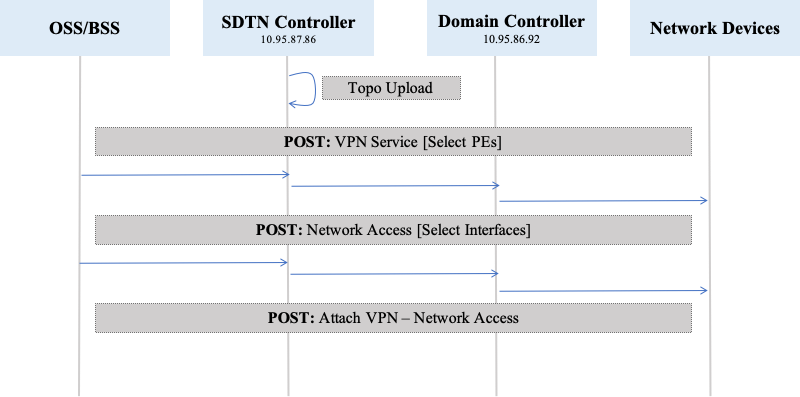
\includegraphics{WORKFLOW.png}}
\caption{Example of a figure caption.}
\label{fig1}
\end{figure}


\begin{figure}[!h]
\centerline{\includegraphics{ARCHITECTURE.png}}
\caption{Example of a figure caption.}
\label{fig1}
\end{figure}

The Layer 3 Virtual Private Network (VPN) service defined in RFC 4364 provides a multipoint, routed service to the customer over an IP/MPLS core. 
L3NM \cite{b3} is a Network Model defined in YANG. The L3NMmodel is exposed by network controllers to manage and control the VPN Service configuration. The model describes a VPN Service in the service provider network. It contains especific information to deploy the configuration on the network, such as NE-ID and Interfaces-ID and might include allocated resources such as the Route Targets, Route Distinguishers, VLANs and IP addressing.

The L3NM data model can be used to facilitate communication between the service orchestrator and the SDTN network controller. Also, the SDTN network controller can further include or expand specific information in the  request (i.e. transport LSP binding, Router Targets assignation, routing profiles or encryption). 

\section{TOPOLOGY MODEL}

The proposed control architecture relies on providing different levels of abstraction for each control layer. Therefore, the needs in terms of topology and knowledge of the service provider network differ among components.

In the proposed hierarchy, the service orchestration layer does not need to know about the internals of the network. The authors have proposed a UNI topology model in \cite{b4}. The SDTN controller exposes the set of nodes. L3 VPN services can be requested adding as attachment points the nodes. For that aim, the UNI topology builds the network data model defined in the "ietf-network" module, augmenting the nodes with service-attachment points.

\section{EXPERIMENTAL VALIDATION}

The experimental set-up simulates an IP/MPLS network scenario, where the data plane consists of two interconnected routers acting as PE devices. Every router has two cards of 10x10G interfaces but only two access client-facing ports (1/1/c10/1 and 1/1/c11/2 in each router) can be used to connect customers. Each port has been configured to support Dot1Q ethernet encapsulation, so several services can be attached to the same physical port, using different VLAN-IDs. The control plane is formed by two pieces:
\begin{itemize}
    \item An SDTN controller is developed by Telefonica. 
    \item A commercial IPSDNc connected to the routers
\end{itemize}
As the SDTN has an E2E view, all the services creation requests must be received by the SDTN, processed, expanded and forwarded using RESTCONF/YANG to the SDN controllers. The communication between the routers and the SDNc is based on NETCONF/YANG. 

The first goal to be achieved was to retrieve the UNI-Topology to determine the available interfaces on the network. One of the service attachment points (by node in the VPN) retrieved  in the UNI-topology must be selected as a service end-point. After that, an End-to-End L3VPN between the selected nodes must be established. So, the SDTN controller will provision the service using RESTCONF + IETF L3NM requests to the IP SDNc. Several scenarios where tested:
\begin{itemize}
    \item All the network parameter defined by the user . 
    \itme RD+RT automatically assigned by the SDTN. 
    \item RD+RT+VLANs automatically assigned by the SDTN
\end{itemize}

The full E2E L3VPN service establishment process is shown in the \ref{fig1} First, the figure shows the RESTCONF request of the L3VPN service creation, how this is received by SDTN Controller, passed to SDNc and accepted by both (step 1). Once the L3VPN service has been created, it is needed to create the desired IE Profiles and VPN Nodes for the service. Steps 2 and 3 of Fig. 1 show the traces of the creation process of one IE Profile and one VPN Node, respectively, for the L3VPN service in SDNc and SDTN Controller.

\section{CONCLUSIONS}

This work demonstrates for the first time two key aspects for network operators in practical scenarios: the mapping between topologies and L3 services, and,  the provisioning of L3 services with L3SM and L3NM interfaces. To do so, this work  implements for the first time L3NM and UNI topology IETF contributions. Finally, the work demonstrates that such automation with current standards and validates the implementation against a commercial SDN controller

\section*{Acknowledgment}
This work was supported partially by the European Commission H2020-ICT-2016-2 METRO-HAUL project (G. A. 761727) and Spanish AURORAS (RTI2018-099178).

\begin{thebibliography}{00}
\bibitem{b1} D. Kreutz, et al., “Software-Defined Networking: A Comprehensive Survey”, Proc. of the IEEE, Vol. 103, Issue 1, pp. 14- 76, January 2015.
\bibitem{b2} L.M. Contreras, et al, “iFUSION: Standards-based SDN Architecture for Carrier Transport Network”, in Proc. of the IEEE CSCN, October 2019.
\bibitem{b3} Aguado, a., et al (2020). draft-ietf-opsawg-l3sm-l3nm-01 -A Layer 3 VPN Network YANG Model. [online] Tools.ietf.org. Available at: https://tools.ietf.org/html/draft-ietf-opsawg-l3sm-l3nm-01 [Accessed 2 Jan. 2020].
\bibitem{b4} Gonzalez de Dios, O., et al (2020). draft-ogondio-opsawg-uni-topology-00 - A YANG Model for User-Network Interface (UNI) Topologies. [online] Tools.ietf.org. Available at: https://tools.ietf.org/html/draft-ogondio-opsawg-uni-topology-00 [Accessed 2 Jan. 2020]
\end{thebibliography}

\end{document}
